\pdfminorversion=4
\documentclass[aspectratio=169]{beamer}

\mode<presentation>
{
  \usetheme{default}
  \usecolortheme{default}
  \usefonttheme{default}
  \setbeamertemplate{navigation symbols}{}
  \setbeamertemplate{caption}[numbered]
  \setbeamertemplate{footline}[frame number]  % or "page number"
  \setbeamercolor{frametitle}{fg=white}
  \setbeamercolor{footline}{fg=black}
} 

\usepackage[english]{babel}
\usepackage[utf8x]{inputenc}
\usepackage{tikz}
\usepackage{courier}
\usepackage{array}
\usepackage{bold-extra}
\usepackage{minted}
\usepackage[thicklines]{cancel}
\usepackage{fancyvrb}
\usepackage{tabto}

\xdefinecolor{dianablue}{rgb}{0.18,0.24,0.31}
\xdefinecolor{darkblue}{rgb}{0.1,0.1,0.7}
\xdefinecolor{darkgreen}{rgb}{0,0.5,0}
\xdefinecolor{darkgrey}{rgb}{0.35,0.35,0.35}
\xdefinecolor{darkorange}{rgb}{0.8,0.5,0}
\xdefinecolor{darkred}{rgb}{0.7,0,0}
\definecolor{darkgreen}{rgb}{0,0.6,0}
\definecolor{mauve}{rgb}{0.58,0,0.82}

\title[2018-10-15-adl-workshop-femtocode]{Making your own language: things to think about}
\author{Jim Pivarski}
\institute{Princeton University -- DIANA-HEP}
\date{October 15, 2018}

\usetikzlibrary{shapes.callouts}
\usetikzlibrary{trees}

\begin{document}

\logo{\pgfputat{\pgfxy(0.11, 7.4)}{\pgfbox[right,base]{\tikz{\filldraw[fill=dianablue, draw=none] (0 cm, 0 cm) rectangle (50 cm, 1 cm);}\mbox{\hspace{-8 cm}
\includegraphics[height=1 cm]{princeton-logo-long.png}
\includegraphics[height=1 cm]{diana-hep-logo-long.png}}}}}

\begin{frame}
  \titlepage
\end{frame}

\logo{\pgfputat{\pgfxy(0.11, 7.4)}{\pgfbox[right,base]{\tikz{\filldraw[fill=dianablue, draw=none] (0 cm, 0 cm) rectangle (50 cm, 1 cm);}\mbox{\hspace{-8 cm}
\includegraphics[height=1 cm]{princeton-logo.png}
\includegraphics[height=1 cm]{diana-hep-logo.png}}}}}

% Uncomment these lines for an automatically generated outline.
%\begin{frame}{Outline}
%  \tableofcontents
%\end{frame}

% START START START START START START START START START START START START START

\begin{frame}[fragile]{Domain specific languages}
\large
\vspace{1 cm}
Many data analysts manage to do all or most of their work with the following:

\vspace{0.25 cm}
\begin{center}
\begin{minipage}{0.85\linewidth}
\begin{minted}{sql}
SELECT expr FROM src WHERE expr GROUP BY expr
\end{minted}
\end{minipage}

\vspace{1.5 cm}
\begin{minipage}{0.7\linewidth}
\begin{center}
\uncover<2->{\LARGE Why do we need a full programming language?}
\end{center}
\end{minipage}
\end{center}
\end{frame}

\begin{frame}{Maybe it goes back to origins? 1890 census: the Hollerith machine}
\vspace{0.25 cm}
\begin{center}
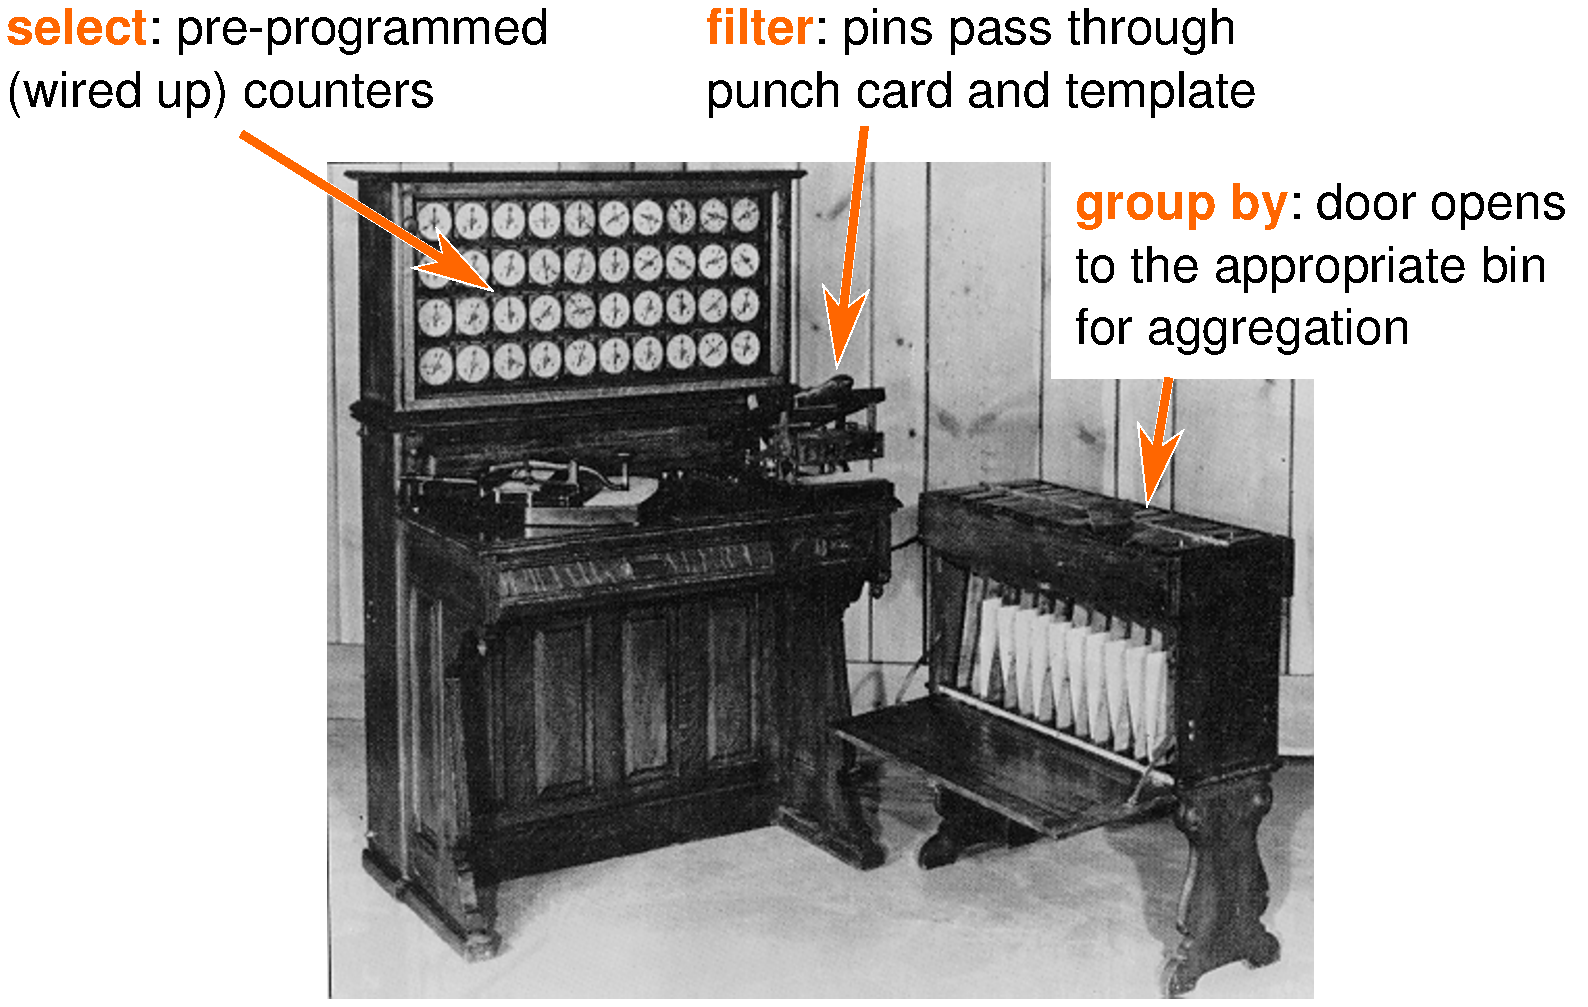
\includegraphics[width=0.83\linewidth]{hh-tabulator.pdf}
\end{center}
\end{frame}

\begin{frame}{Maybe it goes back to origins? 1950's neutron transport MC}
\vspace{0.5 cm}

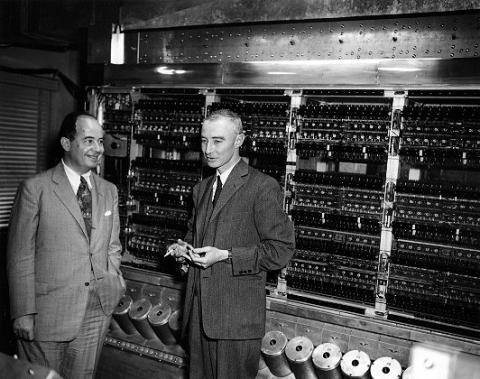
\includegraphics[height=5 cm]{neumann_oppie.jpg} 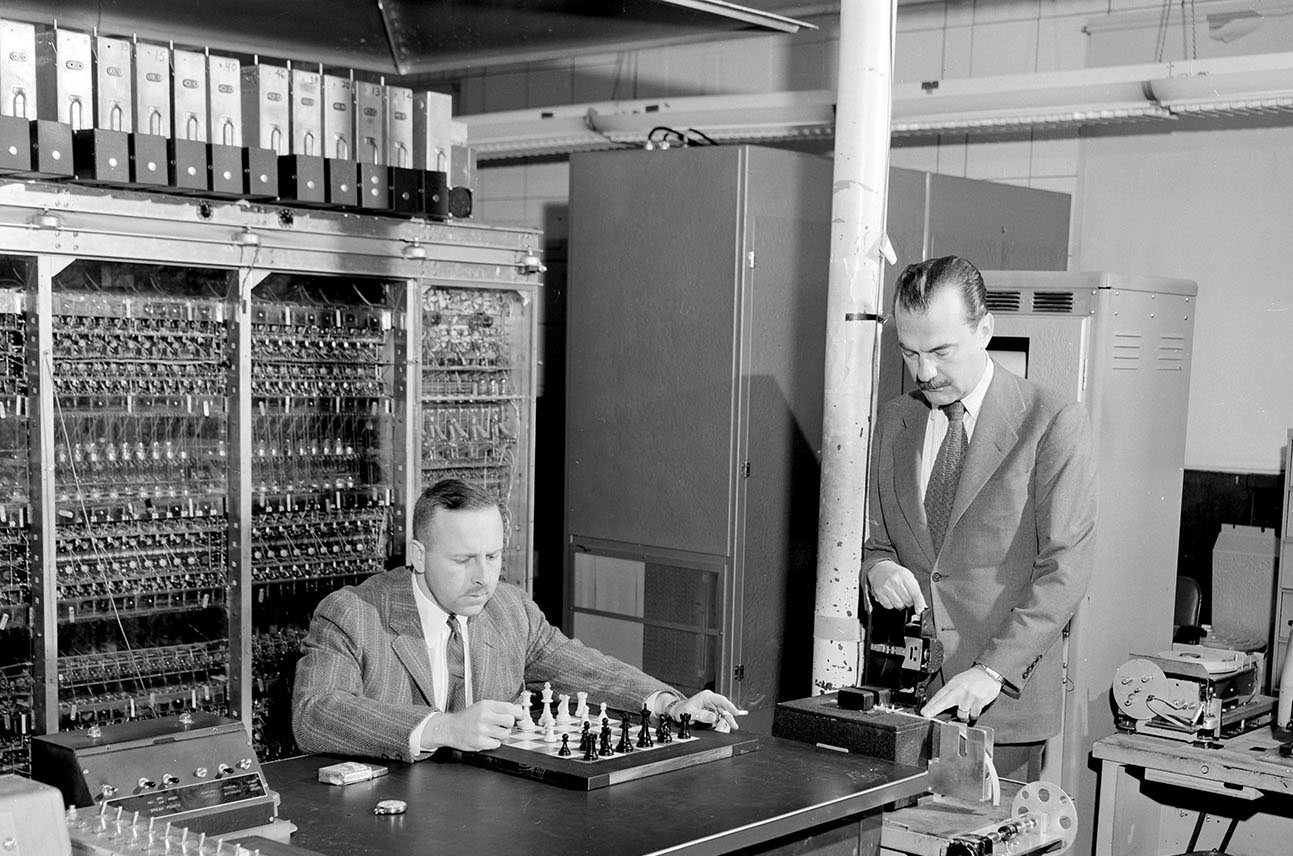
\includegraphics[height=5 cm]{metropolis.jpg}

\begin{center}
\Large {\bf M}etropolis {\bf A}nd {\bf N}eumann {\bf I}nvent {\bf A}wful {\bf C}ontraption
\end{center}
\end{frame}

\begin{frame}{Maybe it goes back to origins?}
\large
\vspace{0.5 cm}

We're accustomed to (ab)using a complete programming environment. Some of our problems strictly need it.

\vspace{0.5 cm}
Particle physics and digital computing ``grew up together.''

\vspace{1 cm}
But what's necessary for Monte Carlo and reconstruction is often overkill for physics analysis.
\end{frame}

\begin{frame}{Shrink-wrapping a language to the problem domain}
\large
\begin{itemize}
\item Fully featured language that makes domain-specific problems easier than general ones?
\end{itemize}

\begin{center}
\textcolor{darkorange}{\bf Fortran77}, \textcolor{darkorange}{\bf Erlang}, \textcolor{darkorange}{\bf awk}, \textcolor{darkorange}{\bf \LaTeX}, \textcolor{darkorange}{\bf PostScript}
\end{center}

\begin{itemize}
\item A limited language that can only be used on domain-specific problems?
\end{itemize}

\begin{center}
\textcolor{darkorange}{\bf SQL92}, \textcolor{darkorange}{\bf HTML4}, \textcolor{darkorange}{\bf regular expressions}, \textcolor{darkorange}{\bf configuration files}
\end{center}
\end{frame}

\begin{frame}{Some terminology}
\large
\vspace{0.5 cm}
\begin{description}\setlength{\itemsep}{0.5 cm}
\item[Turing complete:] can do anything a state machine $+$ infinite ticker tape can do.

\vspace{0.25 cm}
{\normalsize For example, conditional branching $+$ ability to store and retrieve any number of variables. Or the ability of functions to define functions.}

\item[Declarative:] order of expressions does not imply any order of computations.

\vspace{0.25 cm}
{\normalsize For example, SQL SELECT may be computed before or after SQL WHERE. The first element in an HTML document is drawn {\it above} the second, but not necessarily {\it before}. \underline{No} concept of time-order.}

\item[Functional:] computations are defined in terms of functions that accept or return functions, usually with immutable data.

\vspace{0.25 cm}
{\normalsize For example, \small\mintinline{scala}{data.map(ev => ev.muons.maxby(mu => mu.pt))}\normalsize .}
\end{description}
\end{frame}

\begin{frame}[fragile]{Physicists are abusing the word ``declarative;'' let's clarify}
\small
\vspace{0.25 cm}
\begin{center}
\begin{minipage}{0.8\linewidth}
\begin{minted}{python}
def infinite_loop():
    return infinite_loop()

def simple_boolean():
    return False

infinite_loop() and simple_boolean()    # runs forever
simple_boolean() and infinite_loop()    # returns False
\end{minted}
\end{minipage}
\end{center}

\normalsize
\vspace{0.25 cm}
A truly declarative language would be insensitive to order and either always run forever or always short-circuit the boolean logic. Another example:

\small
\begin{center}
\begin{minipage}{0.8\linewidth}
\begin{minted}{python}
x = x + 1     # means that x is +inf, -inf, or NaN
\end{minted}
\end{minipage}
\end{center}

\normalsize
It's hard for a declarative language to be Turing complete.

\vspace{0.5 cm}
When physicists say ``declarative,'' they usually mean ``functional'' or even ``Spark-like.''
\end{frame}

\begin{frame}[fragile]{Spark-like analysis: a pipeline of operations, implicit event loop}
\small
\begin{columns}
\column{1.05\linewidth}
\begin{minted}{python}
physt.h1(
    t.array("muonp4")    # get zero or more muon 4-vectors per event
     .filter(lambda muon: abs(muon.eta) < 1)  # select central muons
     .pairs(same=False)                       # non-duplicate pairs
     .apply(lambda mu1, mu2: mu1 + mu2)       # compute Z candidates
     .maxby(lambda z: z.pt)                   # highest pT per event
     .flatten()                               # ignore empty events
     .mass,                                   # compute mass
    bins=100).plot()
\end{minted}
\end{columns}

\vspace{0.25 cm}
\begin{columns}
\column{0.4\linewidth}
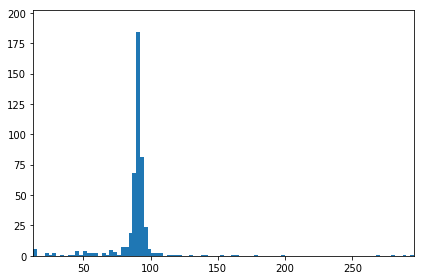
\includegraphics[width=\linewidth]{zpeak.png}

\column{0.6\linewidth}
\begin{uncoverenv}<2->
\normalsize
\hspace{-0.15 cm}This is not even functional: the lambda functions here are pure syntactic sugar for array operations.

\vspace{0.25 cm}
If the goal is to provide a fast, Spark-like interface, we can do that without language features.

\vspace{0.25 cm}
This is working code from awkward-array/uproot; see also ROOT's RDataFrame.

\mbox{ }
\end{uncoverenv}
\end{columns}
\end{frame}

\begin{frame}[fragile]{Functional programming}
\vspace{0.5 cm}
{\bf Higher-order function (a.k.a.\ ``functional'' or ``functor''):} a function that accepts functions as arguments or returns functions.

\vspace{0.5 cm}
\begin{onlyenv}<1>
If the higher-order function only accepts functions as arguments and those arguments are known at ``compile time'' (some processing pass before the high-throughput pass over data), it can be substituted by a loop or parallel loops.

\small
\begin{columns}[t]
\column{0.5\linewidth}
\begin{minted}{python}
x = dataset.filter(
      lambda event:
        event.trigger["Mu24"] &
        event.trigger["DiJet100"])
\end{minted}

\column{0.5\linewidth}
\begin{minted}{python}
x = []
for event in dataset:
  if (event.trigger["Mu24"] &
      event.trigger["DiJet100"]):
    x.append(event)
\end{minted}
\end{columns}
\end{onlyenv}
\begin{onlyenv}<2>
But if a higher-order function doesn't know what function it will be passed until runtime or if it returns functions, it is more powerful than a loop.

\small
\begin{center}
\begin{minipage}{0.8\linewidth}
\begin{minted}{python}
def good(cut):
    return (lambda event: cut(event) &
                          event.trigger["Mu24"])
\end{minted}
\end{minipage}
\end{center}

\vspace{1.2 cm}
\end{onlyenv}
\end{frame}

\begin{frame}[fragile]{Total functional programming}
\vspace{0.25 cm}
A fringe idea in computer science: {\bf total functional programming} solves the

\small
\begin{center}
\begin{minipage}{0.8\linewidth}
\begin{minted}{python}
infinite_loop() and simple_boolean()    # runs forever
simple_boolean() and infinite_loop()    # returns False
\end{minted}
\end{minipage}
\end{center}

\normalsize
problem by forbidding \mintinline{python}{infinite_loop()}. That is, these are non-Turing complete languages--- every function is certain to return a value.

\vspace{0.5 cm}
Combine this with {\bf dependent types}--- type-checking strict enough to distinguish
\begin{itemize}
\item $x$ is an integer
\item $x$ is a non-negative integer
\item $x$ is an integer greater than or equal to 5 and less than 12
\end{itemize}

and it would be possible to write physics expressions without any runtime errors. If it compiles and the input data can be loaded, it will run.
\end{frame}

\begin{frame}[fragile]{Examples from Femtocode (my project in 2016)}
\small
\begin{minted}{python}
>>> propagateTypes("x / y", x=real, y=real)
\end{minted}
{\color{red}
\begin{verbatim}
femtocode.parser.FemtocodeError: Function "/" does not accept
arguments with the given types:

    /(real,
      real)

    Indeterminate form (0 / 0) is possible; constrain with if-else.

Check line:col 1:0 (pos 0):

    x / y
----^
\end{verbatim}}

{\normalsize Can be resolved with a constraint:}

\begin{minted}{python}
>>> propagateTypes("if y != 0: x / y else: None", x=real, y=real)
union(null, real)
\end{minted}
\end{frame}

\begin{frame}[fragile]{Examples from Femtocode (my project in 2016)}
\vspace{0.5 cm}
Predicates and logical operators (``if'', ``and'', ``or'', and ``not'') propagate constraints.

\small
\begin{minted}{python}
>>> propagateTypes("x == 5 and y == 6 and x == y", x=real, y=real)
\end{minted}
{\color{red}
\begin{verbatim}
femtocode.parser.FemtocodeError: Function "==" does not accept
arguments with the given types:

    ==(integer(min=5, max=5),
       integer(min=6, max=6))

    The argument types have no overlap (values can never be equal).

Check line:col 1:27 (pos 27):

    x == 5 and y == 6 and x == y
-------------------------------^
\end{verbatim}}
\end{frame}

\begin{frame}[fragile]{Examples from Femtocode (my project in 2016)}
\vspace{0.5 cm}
Order does not matter (it's {\it actually} declarative)!

\small
\begin{minted}{python}
>>> propagateTypes("x == y and x == 5 and y == 6", x=real, y=real)
\end{minted}
{\color{red}
\begin{verbatim}
femtocode.parser.FemtocodeError: Function "==" does not accept
arguments with the given types:

    ==(integer(min=5, max=5),
       integer(min=6, max=6))

    The argument types have no overlap (values can never be equal).

Check line:col 1:5 (pos 5):

    x == y and x == 5 and y == 6
---------^
\end{verbatim}}
\end{frame}

\begin{frame}{Why am I not working on Femtocode now?}
\large
\vspace{0.5 cm}
``Zero runtime errors'' is a nice feature, but it's not the {\it first} thing we need. Interacting with physicists, I saw that more time is spent dealing with accidental complexity than with runtime errors.

\vspace{0.5 cm}
\begin{center}
\begin{minipage}{0.85\linewidth}
\begin{description}
\item[Accidental complexity] could be replaced with something simpler without losing expressiveness.

\item[Essential complexity] reflects the complexity in the problem the physicist wants to solve.
\end{description}
\end{minipage}
\end{center}

\vspace{1 cm}
``Everything should be made as simple as possible, but not simpler.''

\hfill \it --- Reader's Digest, 1977
\end{frame}

\begin{frame}{High-level versus low-level}
\vspace{0.5 cm}
Python is popular for data analysis because of its terse syntax, simple type system, and reputation of having ``one obvious way to do a thing.''

\vspace{0.5 cm}
It does so by sacrificing performance, which becomes an issue again as physicists scale up their analyses.

\vspace{0.5 cm}
There are many, many solutions to this problem.

\begin{itemize}
\item PyROOT: provides bindings into ROOT and C++ from Python.
\item Numpy: provides array programming constructs like MATLAB.
\item Numba: natively JIT-compiles array-centric Python code to be as fast as C.
\item Cython: mixes C++ and Python (by generating and compiling a C++ extension).
\item pybind11: wraps C++ code as a Python extension.
\end{itemize}
\end{frame}

\begin{frame}[fragile]{The Numpy approach}
\vspace{0.5 cm}
\hfill 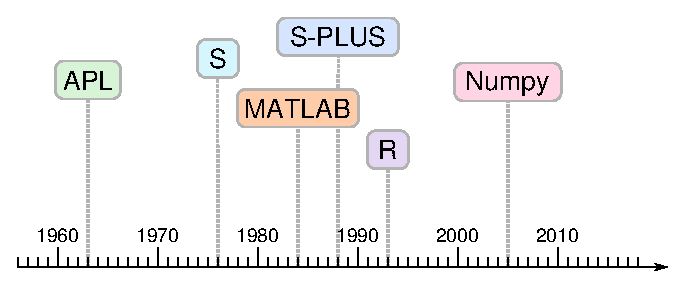
\includegraphics[height=3 cm]{apl-timeline.pdf}

\vspace{-3 cm}
Of all the ``high-level, high-performance'' \\
solutions in Python, Numpy is the most \\
pervasive.

\vspace{0.5 cm}
It's a library that provides a programming \\
model usually seen in specialized analysis \\
languages.

\vspace{0.5 cm}
It models the simplest possible data structures--- arrays of numbers--- with terse syntax for regular operations that can be composed for complex analyses (e.g.\ LIGO).

\small
\begin{center}
\begin{minipage}{0.9\linewidth}
\begin{minted}{python}
indexes    = numpy.argsort(array_pt)   # array of integers
sorted_pt  = array_pt[indexes]         # sorted pT
sorted_eta = array_eta[indexes]        # eta sorted by pT
\end{minted}
\end{minipage}
\end{center}

\normalsize
This won't work for us because our data are not flat arrays, but a simple extension can.
\end{frame}

\begin{frame}{Minimal type system for physics}
\vspace{0.5 cm}

The main issue is that we need nested data structures, like arbitrary length lists of Muon objects, which contain $p_T$ (float), $\eta$ (float), $\phi$ (float), $N_{\mbox{\scriptsize hits}}$ (int), etc.

\large
\begin{description}
\item[{\bf P}rimitives:] numbers and booleans, anything with fixed byte-width; i.e.\ Numpy.

\item[{\bf L}ists:] arbitrary length lists of some type.

\item[{\bf U}nions:] polymorphism; a type like ``electron or muon or tau.''

\item[{\bf R}ecords:] packages of named, typed fields.
\end{description}

\normalsize I've been calling this a ``\textcolor{darkblue}{\bf PLUR}'' type system, and it's as general as the Protocol Buffer, Thrift, Avro, and Parquet data models. But we need one more:

\large
\begin{description}
\item[{\bf P}ointers:] allow nested types to be cousins or ancestors on the type graph (i.e.\ not strictly a tree). This lets the data include cross-references (cousins) and non-tree structures (ancestors).
\end{description}

\normalsize Needed to associate particles to tracks, semileptonic jets to leptons, etc.
\end{frame}

\begin{frame}[fragile]{Representing PLURP data as arrays}
\vspace{0.4 cm}
\textcolor{darkblue}{\Large {\bf L}ists:} represent structure in one array and content elsewhere. Here's an example:

\vspace{0.25 cm}
Logical structure: \tabto{3 cm}{\ttfamily\textcolor{black}{[\textcolor{red}{[}\textcolor{darkblue}{0, 1, 2}], \textcolor{red}{[}], \textcolor{red}{[}\textcolor{darkblue}{3, 4}], \textcolor{red}{[}\textcolor{darkblue}{5, 6, 7, 8, 9}]\textcolor{red}{]}}}

\vspace{0.05 cm}
Offsets:           \tabto{3 cm}{\ttfamily\verb|[|\textcolor{red}{0,}\verb|         |\textcolor{red}{3,}\verb|  |\textcolor{red}{3,}\verb|      |\textcolor{red}{5,}\verb|             |\textcolor{red}{10}\verb|]|}

\vspace{0.05 cm}
Content:           \tabto{3 cm}{\ttfamily\verb|[ |\textcolor{darkblue}{0, 1, 2}\verb|,       |\textcolor{darkblue}{3, 4}\verb|,   |\textcolor{darkblue}{5, 6, 7, 8, 9}\verb|]|}

\vspace{0.05 cm}
Parents:           \tabto{3 cm}{\ttfamily\verb|[ |\textcolor{darkgreen}{0, 0, 0}\verb|        |\textcolor{purple}{2, 2,}\verb|   |\textcolor{darkorange}{3, 3, 3, 3, 3}\verb|]|}

\vspace{0.25 cm}
A ``jagged array'' (content $+$ offsets and/or content $+$ parents) is a basic building block of variable-sized, nested structure.

\vspace{0.5 cm}
\textcolor{darkblue}{\Large {\bf U}nions:} same trick with a ``tags'' array and one ``content'' per type.

\vspace{0.5 cm}
\textcolor{darkblue}{\Large {\bf R}ecords:} one ``content'' for each field. Call it a ``table,'' which becomes a ``jagged table'' if placed in a jagged array; some contents may also be jagged or unions.

\vspace{0.5 cm}
\textcolor{darkblue}{\Large {\bf P}ointers:} reference previously existing arrays, rather than making new ones.
\end{frame}

\begin{frame}{Conventional array programming (arrays of primitives only)}
\vspace{0.5 cm}

{\Large Take inspiration from Numpy array operations\ldots}

\vspace{0.25 cm}
\begin{itemize}\setlength{\itemsep}{0.15 cm}
\item Multidimensional slices: \tabto{5.5 cm}{\small \mintinline{python}{rgb_pixels[0, 50:100, ::3]}}
\item Elementwise operations: \tabto{5.5 cm}{\small \mintinline{python}{all_pz = all_pt * sinh(all_eta)}}
\item Broadcasting: \tabto{5.5 cm}{\small \mintinline{python}{all_phi - 2*pi}}
\item Masking (list compaction): \tabto{5.5 cm}{\small \mintinline{python}{data[trigger & (pt > 40)]}}
\item Fancy indexing (gather/scatter): \tabto{5.5 cm}{\small \mintinline{python}{all_eta[argsort(all_pt)]}}
\item Row/column commutativity \tabto{5.5 cm}{\small \mintinline{python}{table["column"][7]} (row 7 of column array)}

(hides AoS $\leftrightarrow$ SoA): \tabto{5.5 cm}{\small \mintinline{python}{table[7]["column"]} (field of row tuple 7)}
\item Array reduction: \tabto{5.5 cm}{\small \mintinline{python}{array.sum()}} $\to$ scalar
\end{itemize}
\end{frame}

\begin{frame}{Extension to jagged arrays and tables}
\vspace{0.1 cm}
\begin{columns}
\column{1.05\linewidth}
\begin{itemize}\setlength{\itemsep}{0.15 cm}
\item Multidimensional slices: \tabto{5.5 cm}{\small \mintinline{python}{events["jets"][:, 0]}} $\to$ first jet per event
\item Elementwise operations: \tabto{5.5 cm}{\small \mintinline{python}{jetpt * sinh(jeteta)}} $\to$ \mbox{keep jagged structure\hspace{-1 cm}}
\item Broadcasting: \tabto{5.5 cm}{\small \mintinline{python}{jetphi - metphi}} $\to$ expand {\small \mintinline{python}{metphi}} from

\tabto{5.5 cm}one-per-event to one-per-jet before operation

\item Masking (list compaction): \tabto{5.5 cm}{\small \mintinline{python}{data[trigger]}} $\to$ drop whole events

\tabto{5.5 cm}{\small \mintinline{python}{data[jetpt > 40]}} $\to$ drop jets from events

\item Fancy indexing (gather/scatter): \tabto{5.5 cm}{\small \mintinline{python}{a = argmax(jetpt)}} $\to$ \mbox{\small \mintinline{python}{[[2], [], [1], [4]]}\hspace{-0.5 cm}}

\tabto{5.5 cm}{\small \mintinline{python}{jeteta[a]}} $\to$ \mbox{\small \mintinline{python}{[[3.6], [], [-1.2], [0.4]]}\hspace{-0.5 cm}}

\item Row/column commutativity \tabto{5.5 cm}{\small \mintinline{python}{events["jets"]["pt"][7, 1]}} \mbox{(all the same)\hspace{-0.5 cm}}

(project jagged tables to \tabto{5.5 cm}{\small \mintinline{python}{events["jets"][7]["pt"][1]}}

jagged arrays before indexing): \tabto{5.5 cm}{\small \mintinline{python}{events[7]["jets"]["pt"][1]}}

\tabto{5.5 cm}{\small \mintinline{python}{events["jets"][7, 1]["pt"]}}

\tabto{5.5 cm}{\small \mintinline{python}{events[7]["jets"][1]["pt"]}}

\item Jagged array reduction: \tabto{5.5 cm}{\small \mintinline{python}{jetpt.max()}} $\to$ array of max jet $p_T$ per event
\end{itemize}
\end{columns}
\end{frame}

\begin{frame}[fragile]{Solving physics problems with jagged array programming}
\vspace{0.5 cm}
{\bf Problem 1:} Compute the $\phi$ difference between each jet and its event's MET.
\small
\begin{minted}{python}
for event in dataset:
    for jet in event.jets:                  # one per jet minus
        jet.phidiff = jet.phi - event.phi   # one per event
\end{minted}
\normalsize

\vspace{0.5 cm}
{\bf Jagged array solution:} 
\small
\begin{minted}{python}
# because of extended broadcasting rules
events["jets"]["phidiff"] = (
                    events["jets"]["phi"] - events["MET"]["phi"])
\end{minted}
\end{frame}

\begin{frame}[fragile]{Solving physics problems with jagged array programming}
\vspace{0.5 cm}
{\bf Problem 2:} Compute mass of all particles from two collections, subject to a cut.
\small
\begin{minted}{python}
for event in dataset:
    event.leptoquarks = []
    for jet in event.jets:
        for lepton in event.leptons:
            if cut(jet, lepton):
                event.pairs.append(mass(jet, lepton))
\end{minted}
\normalsize

\vspace{0.5 cm}
{\bf Jagged array solution:} 
\small
\begin{minted}{python}
# jagged cross-join makes (jet, lepton) pairs per event
pairs = events["jets"].cross(events["leptons"])

events["leptoquarks"] = mass(pairs[cut(pairs)])
\end{minted}
\end{frame}

\begin{frame}[fragile]{Solving physics problems with jagged array programming}
\vspace{0.25 cm}
{\bf Problem 3:} Find the ``best'' candidate per event or per subcollection.
\small
\begin{minted}{python}
for event in dataset:
    event.best = []
    for leptoquark in leptoquarks:
        if event.best == [] or \
            quality(leptoquark) > quality(event.best[0]):
                event.best = [leptoquark]
\end{minted}
\normalsize

\vspace{0.5 cm}
{\bf Jagged array solution:} 
\small
\begin{minted}{python}
# jagged argmax makes empty lists [] or singleton lists [N]
argbest = quality(events["leptoquarks"]).argmax()

# jagged fancy indexing transforms [] -> [] and [i] -> [sublist[i]]
events["best"] = events["leptoquarks"][argbest]
\end{minted}

\vspace{0.05 cm}
\begin{minted}{python}
# remove empty lists and concatenate singletons by dropping offsets
nonempty_best = events["best"].flatten()
\end{minted}
\end{frame}

\begin{frame}{Like array programming, this does not give up performance}
\vspace{0.3 cm}
\begin{columns}
\column{1.1\linewidth}
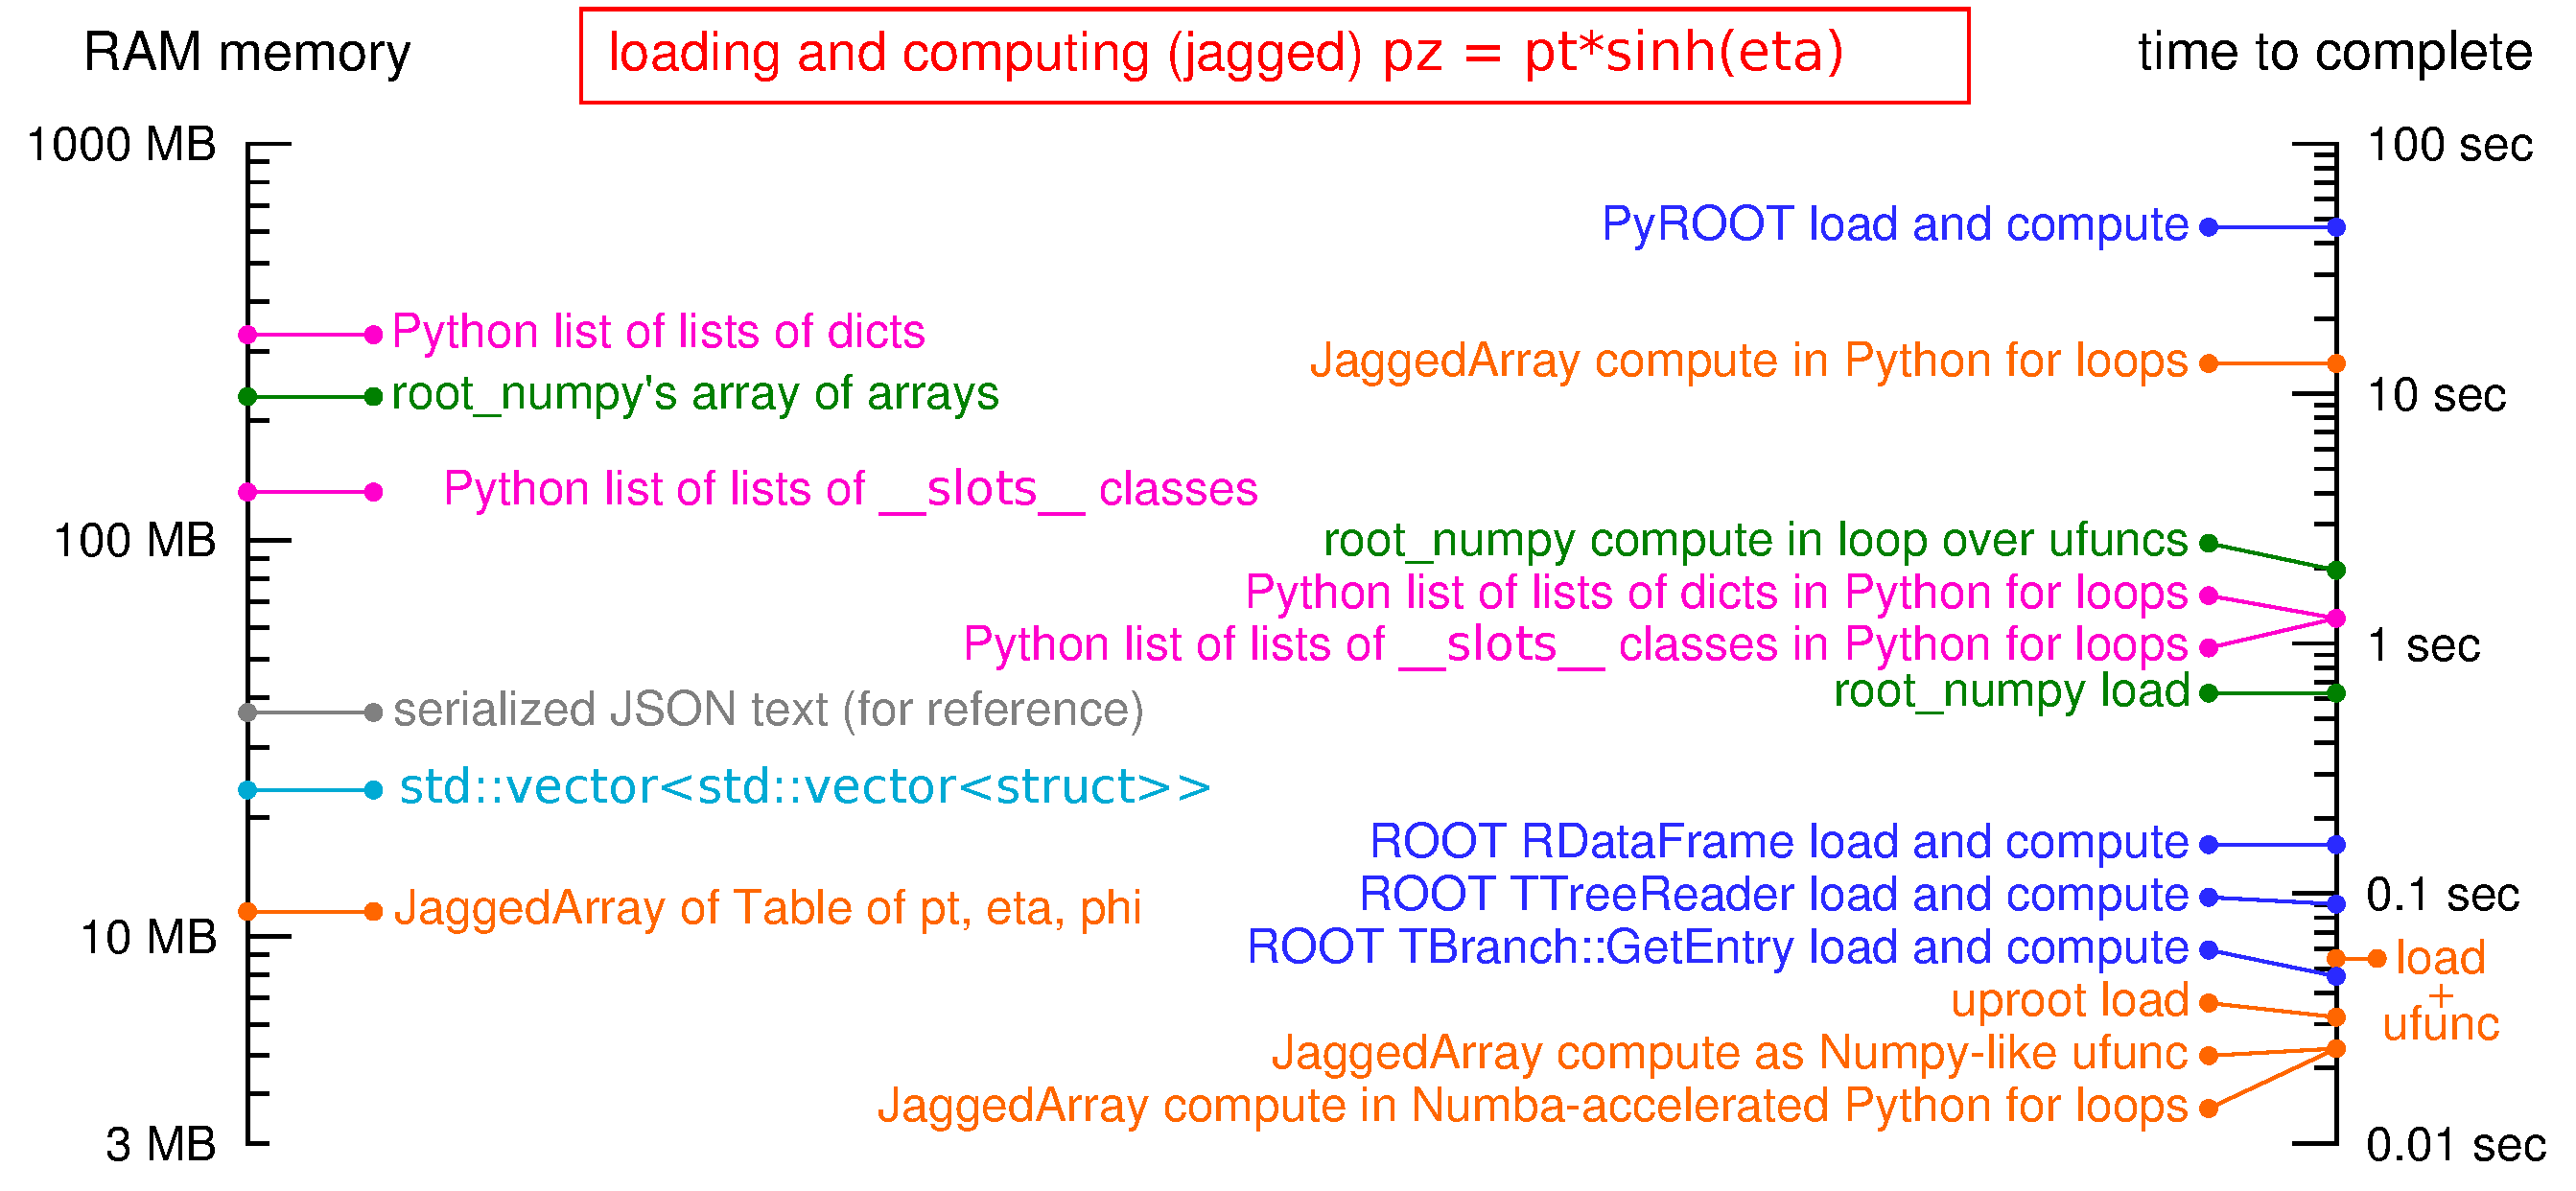
\includegraphics[width=\linewidth]{logscales.pdf}
\end{columns}
\end{frame}

\begin{frame}{awkward-array: a suite of special array classes}
\scriptsize
\vspace{0.45 cm}
\begin{columns}[t]
\column{0.55\linewidth}
\begin{tabular}{p{0.23\linewidth} p{0.55\linewidth} c}
class & purpose & type \\\hline
JaggedArray & representing an array of different-length subarrays, indexed as elements & $[0, \infty) \to T$ \\
ByteJagged- Array & representing an array of different-length subarrays, indexed as bytes & $[0, \inf) \to T$ \\
Table & representing a table of different-typed columns; {\bf mutable: columns can be added or removed} & $\mbox{Table}(T\ldots)$ \\
UnionArray & tagging and indexing elements in arrays to simulate a heterogeneous array & $\mbox{Union}(T\ldots)$ \\
MaskedArray & byte-masking elements of an array as N/A & $\mbox{Option}(T)$ \\
BitMasked- Array & bit-masking elements of an array as N/A & $\mbox{Option}(T)$ \\
IndexedMasked- Array & indexes elements of an array as N/A or as a pointer (content is sparse) & $\mbox{Option}(T)$ \\
ObjectArray & generates objects in an array upon access & opaque\vspace{0.33 cm} \\
\end{tabular}

\column{0.55\linewidth}
\mbox{\hspace{0.95 cm}\begin{tabular}{p{0.2\linewidth} p{0.47\linewidth} c}
class & purpose & type \\\hline
IndexedArray & indexes elements of an array as a pointer by index position & $T$ \\
ByteIndexed- Array & indexes elements of an array as a pointer by byte position & $T$ \\
SparseArray & represents an array storing only elements whose values is not a default value (such as zero); in a sense, the opposite of IndexedArray & $T$ \\
ChunkedArray & logically concatenates discontiguous chunks into one big array; chunk sizes might be known or unknown; appendable & $T$ \\
Appendable- Array & allocates array chunks to append or extend a Numpy array; {\bf mutable: number of rows can grow; restricted: Numpy content only} & $T$ \\
VirtualArray & generates an array upon first access, then caches & $T$ \\
\end{tabular}\hspace{-0.25 cm}}
\end{columns}
\end{frame}

\begin{frame}[fragile]{But this is not a language}
\vspace{0.5 cm}

\begin{columns}
\column{1.035\linewidth}
Array programming requires many temporary variables (or repetition), which introduces an accidental complexity of its own (look at a LIGO analysis!).
\end{columns}

\vspace{0.75 cm}
\begin{columns}[t]
\column{0.45\linewidth}
\underline{Array programming style}

\scriptsize
\vspace{\baselineskip}
\begin{minted}{python}
muonp4    = t.array("muonp4")
muonp4cut = muonp4[abs(muonp4["eta"]) < 1]
muonpairs = muonp4cut.pairs(same=False)
zcands    = muonpairs._0 + muonpairs._1
bestz     = zcands[zcands.pt.argmax()]
bestzflat = bestz.flatten()
masses    = bestzflat.mass
physt.h1(masses, bins=100).plot()
\end{minted}

\column{0.53\linewidth}
\underline{Functional programming sugar}

\scriptsize
\begin{minted}{python}
physt.h1(
    t.array("muonp4")
     .filter(lambda muon: abs(muon.eta) < 1)
     .pairs(same=False)
     .apply(lambda mu1, mu2: mu1 + mu2)
     .maxby(lambda z: z.pt)
     .flatten()
     .mass,
    bins=100).plot()
\end{minted}
\end{columns}

\vspace{0.75 cm}
\begin{columns}
\column{1.035\linewidth}
It's very easy to hide under a functional style (literally 8 lines of code). But that doesn't change the fact that it's strictly evaluated, forcing users to think about order of operations and memory management.
\end{columns}
\end{frame}

\begin{frame}{Suggestion: build a language over awkward-arrays}
\large
\vspace{0.5 cm}
A language consists of
\begin{itemize}
\item a parser
\item a type system
\item optional type checking/inference
\item ``lowering'' to an execution environment
\item an execution engine
\end{itemize}

\vspace{0.5 cm}
The awkward-array library is the last survivor of the Femtocode project: just the execution engine.

\vspace{0.5 cm}
As an execution engine, it's fast, versatile, and suited to particle physics. Everything resolves to array operations, not event-by-event calculations, which are portable to vector processors like GPUs. (An original aim of Femtocode was to be CPU/GPU agnostic.)
\end{frame}

\begin{frame}{Python is a good environment for building languages}
\vspace{0.5 cm}
Language development was once dominated by LISP because of its dynamic typing and simple data structures.

\vspace{0.5 cm}
PLY (Python Lex-Yacc) is a tokenizer-parser generator in pure Python for a reasonably general class of languages (LALR(1), which includes C, Python, and Java).

\vspace{0.5 cm}
Even if you're writing a type-safe language (for numerical processing, you should), it's easier to express the recursive rules for type checking and abstract syntax tree transformations without statically checked types.
\end{frame}

\begin{frame}{Steps in compilation}
\vspace{0.35 cm}

\begin{enumerate}
\item \textcolor{darkblue}{Tokenize:} turn the source code string into a sequence of tokens. For example,

\vspace{0.15 cm}
\mbox{ } \hfill \texttt{\small if (x > 0) \{ x**2 \} else \{ -x**2 \}} \hfill \mbox{ }

\vspace{0.15 cm}
becomes \fbox{\texttt{\scriptsize if}} \fbox{\texttt{\scriptsize (}} \fbox{\texttt{\scriptsize x}} \fbox{\texttt{\scriptsize >}} \fbox{\texttt{\scriptsize 0}} \fbox{\texttt{\scriptsize )}} \fbox{\texttt{\scriptsize \{}} \fbox{\texttt{\scriptsize x}} \fbox{\texttt{\scriptsize **}} \fbox{\texttt{\scriptsize 2}} \fbox{\texttt{\scriptsize \}}} \fbox{\texttt{\scriptsize else}} \fbox{\texttt{\scriptsize \{}} \fbox{\texttt{\scriptsize -}} \fbox{\texttt{\scriptsize x}} \fbox{\texttt{\scriptsize **}} \fbox{\texttt{\scriptsize 2}} \fbox{\texttt{\scriptsize \}}}.

\item \textcolor{darkblue}{Parse:} apply rules like \fbox{\texttt{\scriptsize x}} \fbox{\texttt{\scriptsize **}} \fbox{\texttt{\scriptsize 2}} becomes\begin{tikzpicture}[edge from parent fork right,grow=east,level 1/.style={sibling distance=0.5 cm},baseline=(AA.base)]
\node(AA) {\texttt{**}}
child { node {\texttt{2}} }
child { node {\texttt{x}} };
\end{tikzpicture} and

\fbox{\scriptsize predicate} \fbox{\scriptsize\{} \fbox{\scriptsize consequent} \fbox{\scriptsize\}} \fbox{\scriptsize else} \fbox{\scriptsize\{} \fbox{\scriptsize alternate} \fbox{\scriptsize\}} becomes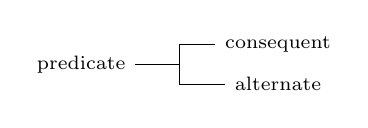
\begin{tikzpicture}[edge from parent fork right,grow=east,level 1/.style={sibling distance=0.5 cm,level distance=2.5 cm},baseline=(AA.base)]
\node(AA) {\scriptsize predicate}
child { node {\scriptsize alternate} }
child { node {\scriptsize consequent} };
\end{tikzpicture}

\item \textcolor{darkblue}{Abstract syntax tree (AST):} data structure from parsing, sometimes transformed to a new tree to add context.

\item \textcolor{darkblue}{Type checking/inference:} adding type attributes to AST nodes from context.

\item \textcolor{darkblue}{Lowering:} transforming AST to another language, such as a sequence of hardware instructions (``compilation''), LLVM Intermediate Representation, or another human-readable language like C++ or Javascript (``transpilation'').
\end{enumerate}
\end{frame}

\begin{frame}{What PLY does for you}
\vspace{0.5 cm}
You supply regular expressions and maybe executable code to identify the next token; PLY repeatedly applies it to tokenize.

\vspace{0.5 cm}
You supply declarative rules that identify groups of tokens and an arbitrary function for the transformation. PLY handles the push-shift steps in the LALR(1) algorithm.

\vspace{0.5 cm}
PLY doesn't make an AST for you; your functions have the freedom to define such a tree (but you {\it should!}).

\vspace{0.5 cm}
I have some code to turn syntax in Backus-Naur form (a declarative grammar) into PLY rules, which makes short work of what you usually want to do.
\end{frame}

\begin{frame}[fragile]{Example of Backus-Naur form: the C programming language}
\fontsize{5}{0}\selectfont
\begin{columns}[t]
\column{0.33\linewidth}
\begin{verbatim}
<trans-unit> ::= {<ext-decl>}*
<ext-decl> ::= <fcn-def> | <decl>
<fcn-def> ::= {<decl-spec>}* <declr>
  {<decl>}* <cmpnd-stmt>
<decl-spec> ::= <storage-class-spec>
  | <type-spec> | <type-qual>
<storage-class-spec> ::= auto | register
  | static | extern | typedef
<type-spec> ::= void | char | short | int
  | long | float | double | signed | unsigned
  | <struct-or-union-spec> | <enum-spec>
  | <typedef-name>
<struct-or-union-spec> ::= <struct-or-union>
  <ident> {{<struct-decl>}+ } |
  <struct-or-union> {{<struct-decl>}+ } |
  <struct-or-union> <ident>
<struct-or-union> ::= struct | union
<struct-decl> ::= {<spec-qual>}*
  <struct-declr-list>
<spec-qual> ::= <type-spec> | <type-qual>
<struct-declr-list> ::= <struct-declr> |
  <struct-declr-list> , <struct-declr>
<struct-declr> ::= <declr> | <declr>
  : <const-expr> | : <const-expr>
<declr> ::= {<pointer>}? <direct-declr>
<pointer> ::= * {<type-qual>}* {<pointer>}?
<type-qual> ::= const | volatile
<direct-declr> ::= <ident> | ( <declr> )
  | <direct-declr> [ {<const-expr>}? ]
  | <direct-declr> ( <param-type-list> )
  | <direct-declr> ( {<ident>}* )
<const-expr> ::= <cond-expr>
<cond-expr> ::= <logical-or-expr> |
  <logical-or-expr> ? <expr> : <cond-expr>
<logical-or-expr> ::= <logical-and-expr> |
  <logical-or-expr> || <logical-and-expr>
<logical-and-expr> ::= <inclusive-or-expr> |
  <logical-and-expr> && <inclusive-or-expr>
\end{verbatim}

\column{0.36\linewidth}
\begin{verbatim}
<inclusive-or-expr> ::= <exclusive-or-expr> |
  <inclusive-or-expr> | <exclusive-or-expr>
<exclusive-or-expr> ::= <and-expr> |
  <exclusive-or-expr> ^ <and-expr>
<and-expr> ::= <equality-expr> | <and-expr>
  & <equality-expr>
<equality-expr> ::= <rel-expr> | <equality-expr>
  == <rel-expr> | <equality-expr> != <rel-expr>
<rel-expr> ::=
  <shift-expr> | <rel-expr> < <shift-expr> |
  <rel-expr> > <shift-expr> | <rel-expr> <=
  <shift-expr> | <rel-expr> >= <shift-expr>
<shift-expr> ::= <add-expr> | <shift-expr> <<
  <add-expr> | <shift-expr> >> <add-expr>
<add-expr> ::= <mul-expr> | <add-expr> +
  <mul-expr> | <add-expr> - <mul-expr>
<mul-expr> ::= <cast-expr> | <mul-expr> *
  <cast-expr> | <mul-expr> / <cast-expr> |
  <mul-expr> % <cast-expr>
<cast-expr> ::= <unary-expr> | ( <type-name> )
  <cast-expr>
<unary-expr> ::= <post-expr> | ++ <unary-expr> |
  -- <unary-expr> | <unary-operator> <cast-expr>
  | sizeof <unary-expr> | sizeof <type-name>
<post-expr> ::= <primary-expr> | <post-expr>
  [ <expr> ] | <post-expr> ( {<assign-expr>}* )
  | <post-expr> . <ident> | <post-expr> ->
  <ident> | <post-expr> ++ | <post-expr> --
<primary-expr> ::= <ident> | <const> | <string>
  | ( <expr> )
<const> ::= <integer-const> | <character-const>
  | <floating-const> | <enumeration-const>
<expr> ::= <assign-expr> | <expr> , <assign-expr>
<assign-expr> ::= <cond-expr> | <unary-expr>
  <assignment-operator> <assign-expr>
<assignment-operator> ::= = | *= | /= | %= | +=
  | -= | <<= | >>= | &= | ^= | |=
\end{verbatim}

\column{0.36\linewidth}
\begin{verbatim}
<unary-operator> ::= & | * | + | - | ~ | !
<type-name> ::= {<spec-qual>}+ {<abstr-declr>}?
<param-type-list> ::= <param-list> |
  <param-list> , ...
<param-list> ::= <param-decl> | <param-list> ,
  <param-decl>
<param-decl> ::= {<decl-spec>}+ <declr> |
  {<decl-spec>}+ <abstr-declr> | {<decl-spec>}+
<abstr-declr> ::= <pointer> | <pointer>
  <direct-abstr-declr> | <direct-abstr-declr>
<direct-abstr-declr> ::=  ( <abstr-declr> ) |
  {<direct-abstr-declr>}? [ {<const-expr>}? ] |
  {<direct-abstr-declr>}? ( {<param-type-list>}? )
<enum-spec> ::= enum <ident> { <enum-list> }
  | enum { <enum-list> } | enum <ident>
<enum-list> ::= <enum> | <enum-list> , <enum>
<enum> ::= <ident> | <ident> = <const-expr>
<typedef-name> ::= <ident>
<decl> ::=  {<decl-spec>}+ {<init-declr>}* ;
<init-declr> ::= <declr> | <declr> = <init>
<init> ::= <assign-expr> | { <init-list> } |
  { <init-list> , }
<init-list> ::= <init> | <init-list> , <init>
<cmpnd-stmt> ::= { {<decl>}* {<stmt>}* }
<stmt> ::= <labeled-stmt> | <expr-stmt> |
  <cmpnd-stmt> | <sel-stmt> | <iter-stmt>
  | <jump-stmt>
<labeled-stmt> ::= <ident> : <stmt> | case
  <const-expr> : <stmt> | default : <stmt>
<expr-stmt> ::= {<expr>}? ;
<sel-stmt> ::= if ( <expr> ) <stmt> | if ( <expr>
  ) <stmt> else <stmt> | switch ( <expr> ) <stmt>
<iter-stmt> ::= while ( <expr> ) <stmt> | do
  <stmt> while ( <expr> ) ; | for ( {<expr>}? ;
  {<expr>}? ; {<expr>}? ) <stmt>
<jump-stmt> ::= goto <ident> ; | continue ; |
  break ; | return {<expr>}? ;
\end{verbatim}
\end{columns}
\end{frame}

\begin{frame}[fragile]{Example of tokenizing/parsing (generated from Backus-Naur)}
\vspace{0.25 cm}
\begin{columns}[t]
\column{0.5\linewidth}
{\large \underline{From the tokenizer}}

\tiny
\begin{minted}{python}
def t_DEC_NUMBER(t):
    r"(0+|[1-9][0-9]*)"
    t.value = int(t.value), kwds(t.lexer, len(t.value))
    return t
tokens.append("DEC_NUMBER")

def t_NAME(t):
    r"[a-zA-Z_][a-zA-Z0-9_]*"
    t.type = reserved.get(t.value, "NAME")
    t.value = t.value, kwds(t.lexer, len(t.value))
    return t
tokens.append("NAME")

def t_EQEQUAL(t):
    r"\=\="
    t.value = t.value, kwds(t.lexer, len(t.value))
    return t

def t_EQUAL(t):
    r"\="
    t.value = t.value, kwds(t.lexer, len(t.value))
    return t

def t_comment(t):
    r"[ ]*\043[^\n]*"  # \043 is "#"
    pass

t_ignore = " \t\f"
\end{minted}

\column{0.5\linewidth}
{\large \underline{From the parser}}

\tiny
\begin{minted}{python}
# arith_expr: term (('+' | '-') term)*
def p_arith_expr_1(p):
    '''arith_expr : term'''
    #                  1
    p[0] = p[1]
def p_arith_expr_2(p):
    '''arith_expr : term arith_expr_star'''
    #                  1               2
    p[0] = unwrap_left_associative([p[1]] + p[2],
                                   alt=len(p[2]) > 2)

def p_arith_expr_star_1(p):
    '''arith_expr_star : PLUS term'''
    #                       1    2
    p[0] = [Add(**p[1][1]), p[2]]
def p_arith_expr_star_2(p):
    '''arith_expr_star : MINUS term'''
    #                        1    2
    p[0] = [Sub(**p[1][1]), p[2]]
def p_arith_expr_star_3(p):
    '''arith_expr_star : arith_expr_star PLUS term'''
    #                                  1    2    3
    p[0] = p[1] + [Add(**p[2][1]), p[3]]
def p_arith_expr_star_4(p):
    '''arith_expr_star : arith_expr_star MINUS term'''
    #                                  1     2    3
    p[0] = p[1] + [Sub(**p[2][1]), p[3]]
\end{minted}
\end{columns}
\end{frame}

\begin{frame}{Type checking/inference}
\vspace{0.35 cm}
Apply type inference rules to propagate types from knowns (literal constants and function arguments) to unknowns (through expressions to assignments). For example,

\vspace{-0.25 cm}
\[ (e_1: \mbox{int} \wedge e_2: \mbox{int}) \Rightarrow e_1 + e_2: \mbox{int} \]

\vspace{-0.5 cm}
\[ (e_1: \mbox{int} \wedge e_2: \mbox{float}) \Rightarrow e_1 + e_2: \mbox{float} \]

\vspace{-0.5 cm}
\[ (e_1: \mbox{float} \wedge e_2: \mbox{float}) \Rightarrow e_1 + e_2: \mbox{float} \]

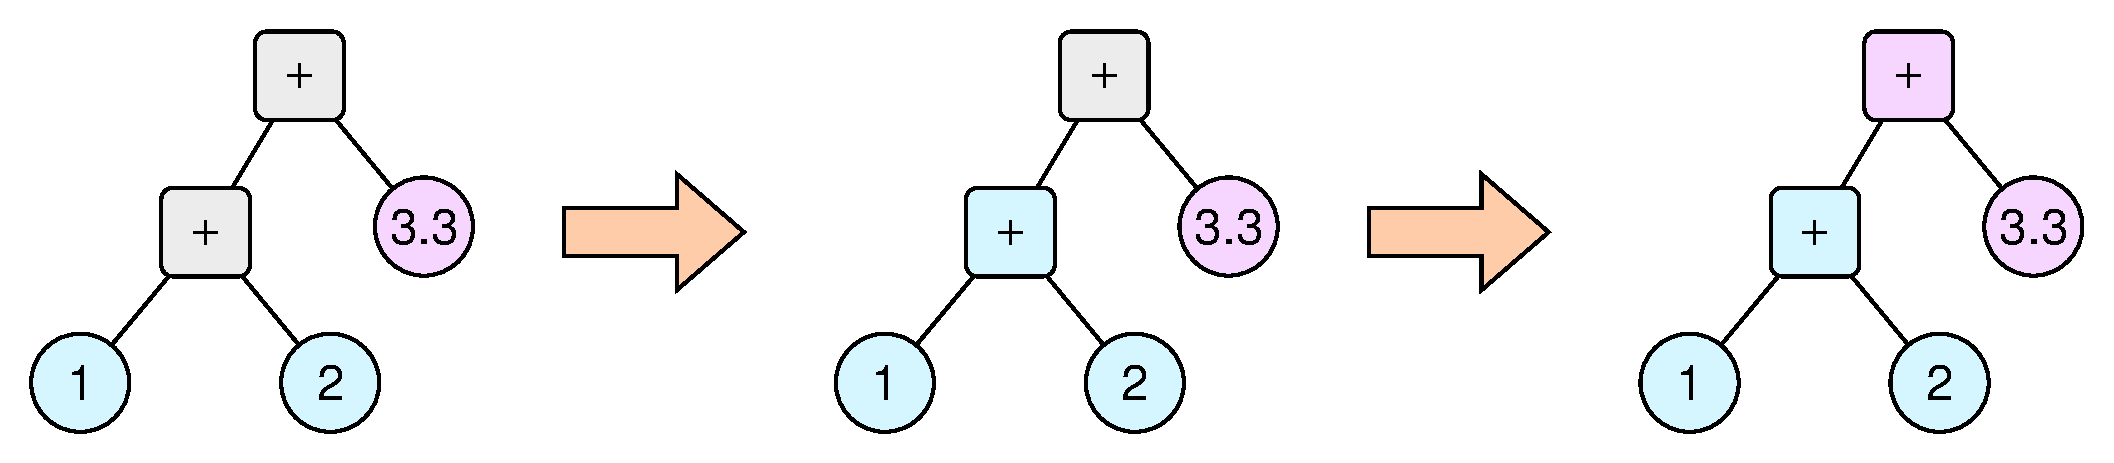
\includegraphics[width=\linewidth]{type-inference.pdf}

\vspace{0.25 cm}
If the inference gets to a point where there are no rules, that's a type error.

\vspace{0.1 cm}
Surviving the type checking pass is a proof that the code will have certain properties.
\end{frame}

\begin{frame}{Lowering}
\vspace{0.5 cm}
\textcolor{darkblue}{Final stage:} turn your AST into another language for someone else to deal with.

\vspace{0.25 cm}
\begin{itemize}\setlength{\itemsep}{0.5 cm}
\item \textcolor{darkorange}{\bf Directly emit machine code?} Difficult and hardware-dependent; this is what gcc does (as well as pycparser).

\item \textcolor{darkorange}{\bf Emit LLVM Intermediate Representation (IR)?} Popular these days: a typed assembly language that compiles to machine code with optimization: get Cling's optimizations for free.

\item \textcolor{darkorange}{\bf Write another human-readable language, like C++?} Called ``transpiling,'' this is a perfectly valid technique. Hundreds of languages ``compile to Javascript'' for use in web development.

\vspace{0.25 cm}
Only drawback: if errors occur in the second compilation, they may be hard to debug (different line numbers, variable names), and will be bewildering to the user.
\end{itemize}
\end{frame}

\begin{frame}{Getting back to my suggestion}
\vspace{0.5 cm}
The lowered language could be Python making awkward-array calls.

\vspace{0.5 cm}
Instead of AST $\to$ language, transform your AST $\to$ the Python AST with appropriate function calls. Skipping a second parsing step speeds up compilation, making it suitable for Just-In-Time (JIT) compilation in an interactive environment.

\vspace{0.5 cm}
You can build higher-level types on a simple PLURP type system.

\vspace{0.5 cm}
You get CPU $\leftrightarrow$ GPU independence for free.

\vspace{0.5 cm}
I will be developing and optimizing the awkward-array library; it makes a good factorization between high-level concepts and low-level implementations.
\end{frame}

\begin{frame}{The hardest and most important question}
\huge
\vspace{0.5 cm}
\begin{center}
\begin{minipage}{0.8\linewidth}
\begin{center}
What language features and built-in functions do physicists need?
\end{center}
\end{minipage}
\end{center}
\end{frame}

\end{document}
